\documentclass[11pt]{article}
\newcommand{\FH}{FHIRKA}


\setlength{\textwidth}{6.5in}
\setlength{\textheight}{8.5in}
\setlength{\evensidemargin}{0in}
\setlength{\oddsidemargin}{0in}
\setlength{\topmargin}{0in}

\setlength{\parindent}{0pt}
\setlength{\parskip}{0.1in}

%\usepackage[dvips]{graphicx}

\usepackage{pgfplots,float}
\pgfplotsset{compat=1.11}

\usepackage{amsmath,amssymb,amsthm,epsfig}
\usepackage{enumerate,color,soul}
\def\H2{{{\mathsf H}_2}}
\def\G{{\mathcal G}}
%\input{../vf_def}

\def\serkan#1{\textcolor{blue}{{#1}}}
\def\caleb#1{\textcolor{blue}{{#1}}}
\def\chris#1{\textcolor{blue}{{#1}}}
\def\serkanlast#1{\textcolor{blue}{{#1}}}


\title{Authors' Response to the Referee Comments}
\author{}
\date{}
\begin{document}
\maketitle

We thank the referees {for their detailed reading of the manuscript and their valuable comments}.
 We have incorporated all the changes that the referees have suggested into the revised
manuscript.   We list below the referees' comments, followed by our responses, denoted by \serkan{\textsf{AR}}.  

Also in the revised manuscripts, all the revisions  are highlighted by color blue for the referees to spot them easily.

\section*{Referee \#1}%change this about referee #1

\begin{itemize}
\item My only concern is the fact that the term H2 is used on time-domain
function, which might be inappropriate from a mathematical point of
view?\\[1ex]
\serkan{\textsf{AR}: We agree with the referee that the term $H_2$ is associated with measure in the frequency domain. To clarify this point. we have added a footnote, namely Footnote 4, at the bottom of page 3, explaining the usage.
} 
\end{itemize}

\section*{Referee \#2}

\begin{itemize}
\item The introduction of the paper does not allow to position the problem
accurately even though valuable elements of this positioning are given
in section 3.3. \\ [1ex]
\serkan{\textsf{AR}:  We thank the referee for pointing this out. We have added some of this discussion from Section 3.3 to Introduction now (the second to last paragraph in Introduction) to help resolve this issue.}   

\item Some particular application domains are cited in the beginning without
justification. \\[1ex]
\serkan{\textsf{AR}:  We have added citations as suggested.}  
\item What about the choice of the finite horizon tf ? \\ [1ex]
\serkan{\textsf{AR}: The choice of the finite horizon is  problem and application dependent; however the interpolation conditions hold for any $t_f$. We added a sentence right before Remark 3.2 to state this fact.}

\item Justify the choice of simple poles for the reduced order model. \\ [1ex]
\serkan{\textsf{AR}:  The choice of simple poles was motivated by the infinite horizon $\mathcal{H}_2$ optimal approximation problem and the corresponding interpolation conditions, as in, for example, citations [3,6,7, 11,23] in our manuscript. The interpolatory $\mathcal{H}_2$  approximation has been extended some specific nonlinear dynamical systems as well, such as 
\begin{itemize}
\item   P. Benner and T. Breiten, Interpolation-based $\mathcal{H}_2$-model reduction of
                  bilinear control systems, SIAM Journal on Matrix Analysis and Applications, 2012.
\item  G. Flagg and S. Gugercin,  Multipoint Volterra Series Interpolation and $\mathcal{H}_2$ Optimal Model Reduction of Bilinear Systems, SIAM Journal on Matrix Analysis and Applications, 2015.
\item P. Benner , P. Goyal, and S. Gugercin, $\mathcal{H}_2$-quasi-optimal model order reduction for quadratic-bilinear control systems, SIAM Journal on Matrix Analysis and Applications, 2018.
\end{itemize}
These nonlinear extensions also use the same assumption. It is certainly theoretically possible that an optimal $\mathcal{H}_2$ reduced model can have repeated poles and interpolation conditions have been extended to this case: 
\begin{itemize}
\item P. van Dooren, K. Gallivan, and  P.-A. Absil, 
$\mathcal{H}_2$-Optimal Model Reduction with Higher-Order Poles,
	SIAM Journal on Matrix Analysis and Applications, 2010.
\end{itemize}
However, this situation is rarely observed in practice and for simplicity of the presentation and notation we chose to use simple poles. Also, we note that the full model can have repeated poles. The assumption is only for the reduced model.
}  

\item What is the reference of the existing result given by Theorem 2.1 ? \\ [1ex]
\serkan{\textsf{AR}:  We have added the citation immediately after the theorem.}  

\item Notation are not fixed in the paper. For example H'(s) is the
derivative of H with respect to s. This can be stated at the end of the
introduction section (with all other notations...)\\ [1ex]
\serkan{\textsf{AR}:  We have added a clarification for this notation immediately after Theorem 2.1, which corresponds to the first occurrence of $\bf{H}'(s)$ .} 

\item  Section 2.2 : the 5 introduction lines are very important and can be
used to state the purpose of the paper. \\ [1ex]
\serkan{\textsf{AR}: These five lines state the purpose of infinite horizon optimal model reduction even though what we consider here, i.e., optimal model reduction on a finite horizon, has some similar difficulties. Following the referee's earlier suggestion (the first comment), we have added some more discussion about our approach to  Introduction.}

\item section 3 : the first 5 lines are a "useless repetition" and can be
removed. \\ [1ex]
\serkan{\textsf{AR}:  We have removed these 5 lines and reorganized the beginning of Section 3 as suggested.}


\item Section 3 : lines 6 to 10 can be given as a Remark (important remark!)  \\ [1ex]
\serkan{\textsf{AR}:  We have followed  the referee's recommendation and list these lines as Remark 3.3 now. }

\item Remark 3.2 can be given after the proof of the main result and can be
a part of the discussion of the given result. \\[1ex]
\serkan{\textsf{AR}:  We have moved the remark after the proof as the referee suggested. }

\item Lemma 3.3 : "Let G(s) and Gr(s) be as defined in (3.5) and (3.7)"
instead of "Let G(s) and Gr(s) be as defined in (3.5) and (3.5)" \\ [1ex]
\serkan{\textsf{AR}:  We thank the referee for pointing out this issue. We have addressed it in the revised version.} 

\item Page 8 : (3.18) is one equation no need to (3.19). \\ [1ex]
\serkan{\textsf{AR}:  We thank the referee for pointing out this issue. We have addressed it in the revised version.}

\item The computation of (3.18) is not clear. One can give more details
allowing to obtain such result. \\ [1ex]
\serkan{\textsf{AR}:   We have added more details after Equation (3.18) better explaining these computations.}

\item Sentence after (3.19) : "...in the parentheses in (3.18) and (3.19)"
instead of "...in the parentheses in (3.18) and (3.18)". \\[1ex]
\serkan{\textsf{AR}:  We thank the referee for pointing out this issue. We have addressed it in the revised version.}

\item 3.3 section can be a (concise) part of the introduction of the paper. \\[1ex]
\serkan{\textsf{AR}:  Following the referee's suggestion, we have added the basic points of Section 3.3 to Introduction. However, some of the discussions in  Section 3.3 depend on the main theoretical results of the paper and it is hard to discuss them in Introduction without these theoretical details. Therefore, as the referee suggested, our motivation to Introduction only highlight the main points of the analysis.}

\item Section 4 : should state how to use the main result in constructing
the reduced order model which is not the case in the current version.\\
\serkan{\textsf{AR}:  This comment was not very clear to us.  Corollaries 4.1 and 4.2, which follow directly from the main result, explain how we are using the optimality conditions to construct the algorithm.  We were not sure what else the referee would like to see explained.}

\item The numerical examples try to show the "supremacy" of the proposed
result which is obviously not the case. Instead, it will be useful to
explain clearly the aim of each numerical experimentation before giving
a clear figure (with only one comparison aim at each time). The given
figures are almost indecipherable !\\[1ex]
\serkan{\textsf{AR}:  We thank the referee for pointing out the difficulties in reading the figures. We have now separated the figures into subplots, making the comparisons easier and hopefully making the figures more clear.
}

\textcolor{blue}{
 For every model and for every reduced order we have tried, FHIRKA has improved whatever initialization method we have used. Even though we have not used the term ``supremacy" specifically, we believe it is fair to say that  FHIRKA outperformed other methods since this is what we have observed in every scenario we have tried. In some cases the improvements were dramatic in some cases less so. However regardless it has produced a lower error. We have excluded some $r$ values not because FHIRKA performed bad. It was simply because other methods has lead to such poor approximations that they should not be used as an initialization.}

\end{itemize}

\section*{Referee \#3}

\begin{itemize}
\item As stated in Remark 3.2, the optimality condition is not directly
expressed by H(s) and Hr(s), but by G(s) and Gr(s), defined by (3.5)
and (3.7).  The reviewer cannot find a physical interpretation of G(s)
and Gr(s).  The authors can comment on the interpretation.\\[1ex]
\serkan{\textsf{AR}:   We have addressed this issue on the revised version  and added Remark 3.2 to precisely address the referee's comment.}

\item In Numerical Simulation, the authors can add some time responses of
the original and reduced-order models.	For example, showing impulse
responses of the models enables readers to understand "practical"
importance of the proposed method.\\[1ex]
\serkan{\textsf{AR}:  We have added a graph showing the time responses for the error for different methods; Figure 4 in the revised version. We have chosen to include the impulse error plot instead of the impulse responses to better illustrate the deviations.  Due to the page limit stated by Automatica, we were able to include only one such figure. For a reference, we are including  two additional graphs here.}
 \begin{figure}[H]
 \centering
   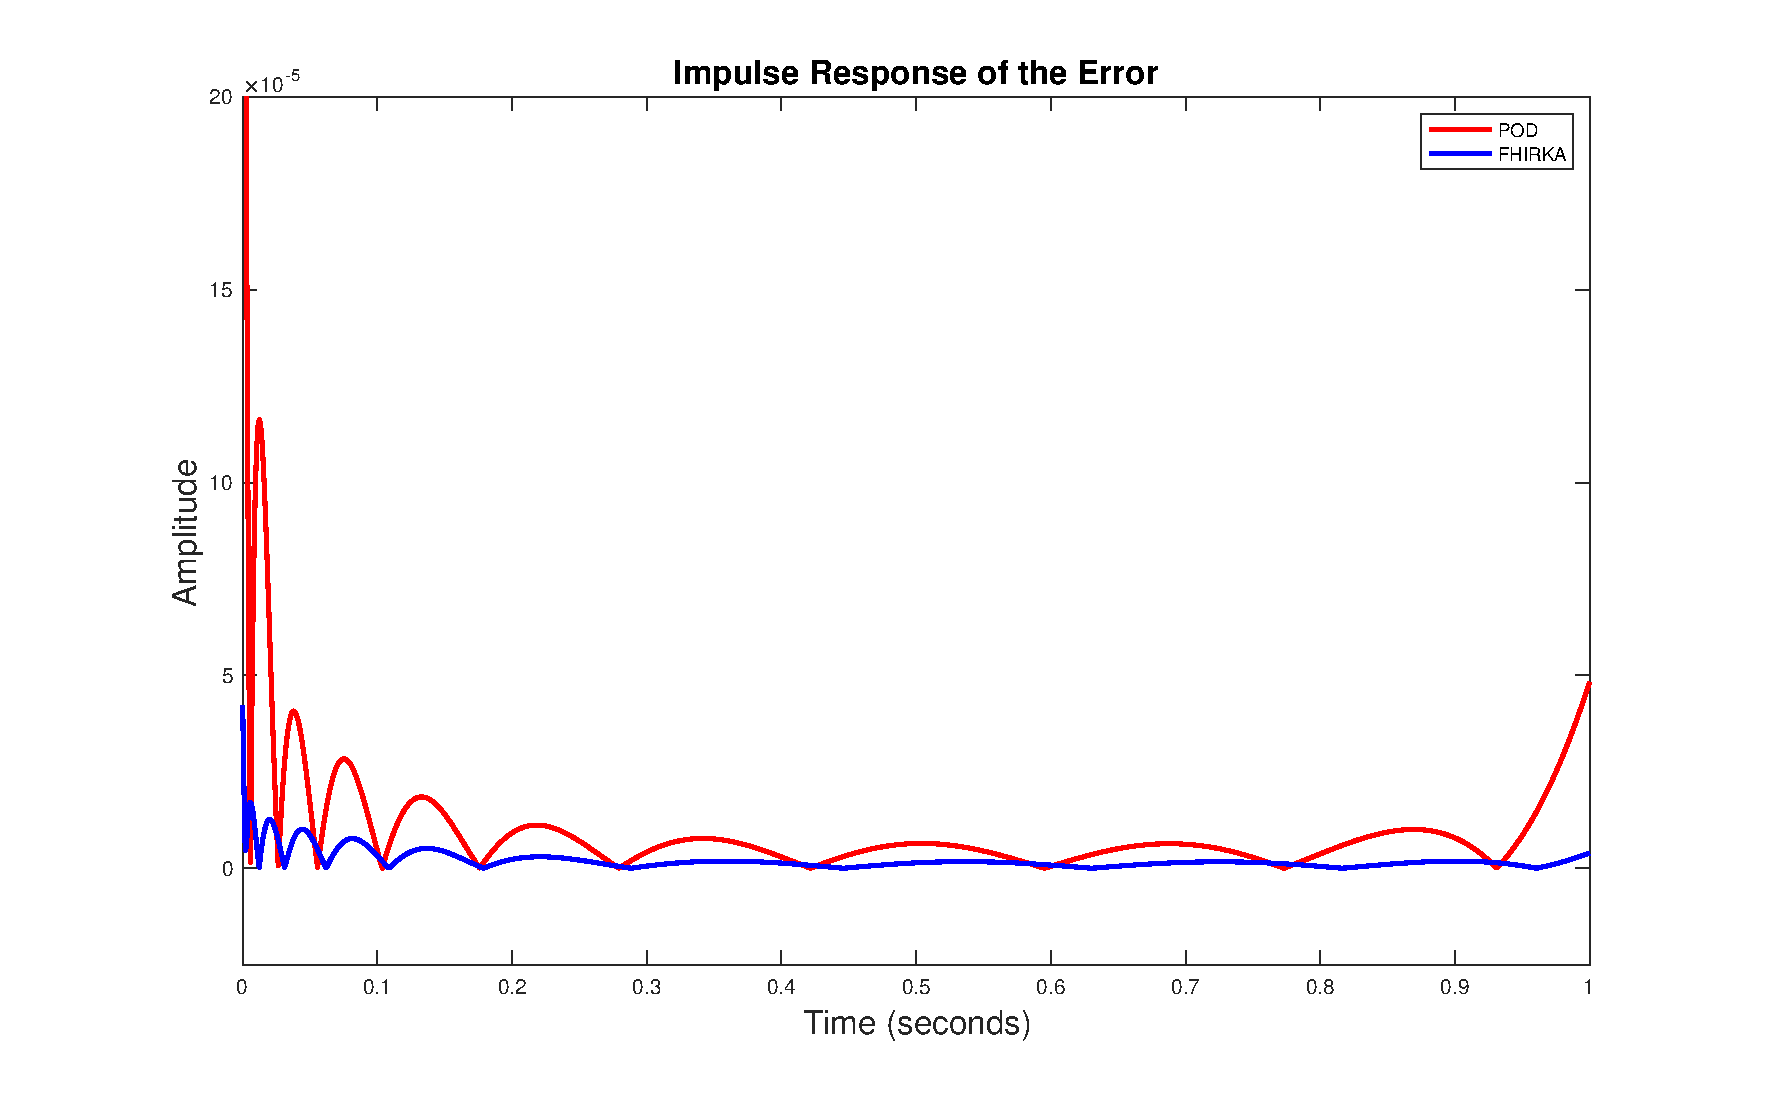
\includegraphics [scale=0.5]{absHeatErrorYlim}
      \caption{POD vs \FH for the heat model\label{fig:impulseHeat}}
 \end{figure}
 \begin{figure}[H]
 \centering
   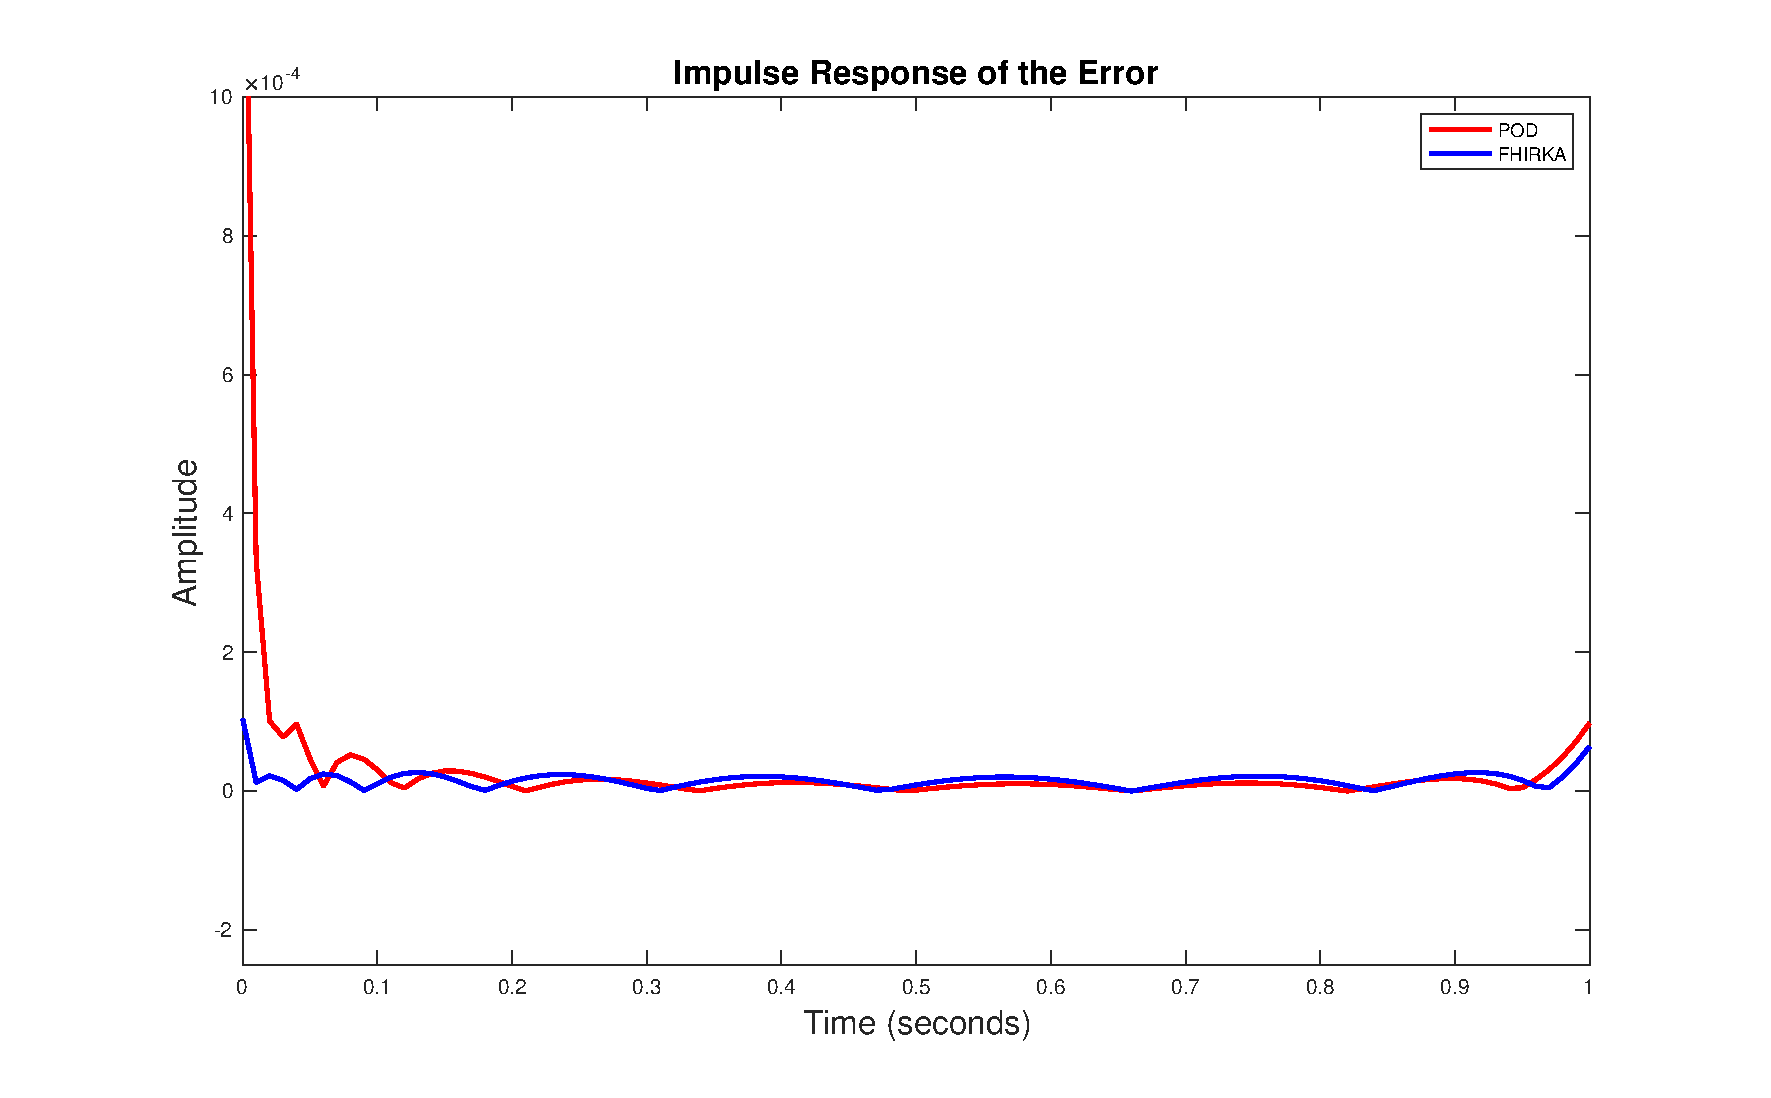
\includegraphics [scale=0.5]{absUNSError}
      \caption{POD vs\  \FH for the unstable model\ \label{fig:impulseUns}}
 \end{figure}



\item  There are some typos in the manuscript.  For example, the statement
"G(s) and Gr(s) be as defined in (3.5) and (3.5)" in Lemma 3.3 should
be corrected. \\[1ex]
\serkan{\textsf{AR}:  We thank the referee for pointing out this issue. We have addressed it in the revised version.}

\end{itemize}

\end{document}